\documentclass[12pt]{article}
\usepackage[utf8]{inputenc}
\usepackage{amsmath,amsfonts,amssymb}
\usepackage{graphicx}
\usepackage{array}
\usepackage{longtable}
\usepackage{multirow}
\usepackage{fancyhdr}
\usepackage{listings}
\usepackage{tikz}
\usepackage{color}
\usepackage{url}

% Custom commands
\newcommand{\highlight}[1]{\textbf{\textit{#1}}}
\newcommand{\code}[1]{\texttt{#1}}

% Page setup
\pagestyle{fancy}
\fancyhf{}
\fancyhead[L]{Complex DVI Test Document}
\fancyhead[R]{\thepage}
\fancyfoot[C]{Generated for dvi-tools testing}

\title{Complex Document Structure for DVI Analysis}
\author{DVI Tools Test Suite}
\date{\today}

\begin{document}

\maketitle

\tableofcontents
\newpage

\section{Introduction}
This document contains various \LaTeX{} constructs to generate a complex DVI file structure for testing the \highlight{dvi-tools} parser and analyzer.

The document includes multiple font sizes, mathematical expressions, tables, lists, and special formatting to stress-test the DVI parsing capabilities.

\section{Typography and Fonts}

\subsection{Font Variations}
\textbf{Bold text}, \textit{italic text}, \texttt{monospace text}, and \textsf{sans-serif text}.

{\tiny Tiny text} {\scriptsize Script size} {\footnotesize Footnote size} {\small Small text} {\normalsize Normal size} {\large Large text} {\Large Larger text} {\LARGE Even larger} {\huge Huge text} {\Huge Massive text}

\subsection{Special Characters and Symbols}
Greek letters: $\alpha \beta \gamma \delta \epsilon \zeta \eta \theta \iota \kappa \lambda \mu \nu \xi \omicron \pi \rho \sigma \tau \upsilon \phi \chi \psi \omega$

Mathematical symbols: $\sum \prod \int \oint \bigcap \bigcup \bigoplus \bigotimes \coprod$

Special characters: \& \% \$ \# \_ \{ \} \textbackslash

\section{Mathematical Expressions}

\subsection{Inline Mathematics}
The quadratic formula is $x = \frac{-b \pm \sqrt{b^2 - 4ac}}{2a}$ where $a \neq 0$.

Einstein's famous equation $E = mc^2$ relates energy and mass.

\subsection{Display Mathematics}
\begin{equation}
\int_{-\infty}^{\infty} e^{-x^2} dx = \sqrt{\pi}
\end{equation}

\begin{align}
\nabla \times \mathbf{E} &= -\frac{\partial \mathbf{B}}{\partial t} \\
\nabla \times \mathbf{B} &= \mu_0\mathbf{J} + \mu_0\epsilon_0\frac{\partial \mathbf{E}}{\partial t} \\
\nabla \cdot \mathbf{E} &= \frac{\rho}{\epsilon_0} \\
\nabla \cdot \mathbf{B} &= 0
\end{align}

Matrix operations:
\begin{equation}
\begin{pmatrix}
a & b & c \\
d & e & f \\
g & h & i
\end{pmatrix}
\begin{pmatrix}
x \\ y \\ z
\end{pmatrix}
=
\begin{pmatrix}
ax + by + cz \\
dx + ey + fz \\
gx + hy + iz
\end{pmatrix}
\end{equation}

\subsection{Complex Mathematical Structures}
\begin{equation}
\sum_{n=0}^{\infty} \frac{x^n}{n!} = e^x = \lim_{n \to \infty} \left(1 + \frac{x}{n}\right)^n
\end{equation}

\begin{equation}
\oint_C \mathbf{F} \cdot d\mathbf{r} = \iint_S (\nabla \times \mathbf{F}) \cdot d\mathbf{S}
\end{equation}

\section{Tables and Arrays}

\subsection{Simple Table}
\begin{center}
\begin{tabular}{|l|c|r|p{3cm}|}
\hline
Left & Center & Right & Paragraph \\
\hline
Item 1 & 100 & \$50.00 & This is a longer text that wraps within the cell \\
Item 2 & 200 & \$75.50 & Another description with multiple words \\
Item 3 & 150 & \$62.25 & Final row with some content \\
\hline
\end{tabular}
\end{center}

\subsection{Complex Table with Multirow and Multicolumn}
\begin{center}
\begin{tabular}{|c|c|c|c|}
\hline
\multicolumn{2}{|c|}{Header Span} & \multicolumn{2}{c|}{Another Span} \\
\hline
Col 1 & Col 2 & Col 3 & Col 4 \\
\hline
\multirow{3}{*}{Vertical Span} & A & B & C \\
\cline{2-4}
& D & E & F \\
\cline{2-4}
& G & H & I \\
\hline
Single & \multicolumn{3}{c|}{Large spanning cell content} \\
\hline
\end{tabular}
\end{center}

\section{Lists and Enumerations}

\subsection{Itemized Lists}
\begin{itemize}
\item First level item
\begin{itemize}
\item Second level item
\begin{itemize}
\item Third level item
\item Another third level
\end{itemize}
\item Back to second level
\end{itemize}
\item Another first level item
\end{itemize}

\subsection{Numbered Lists}
\begin{enumerate}
\item Primary numbered item
\begin{enumerate}
\item Sub-numbered item with $f(x) = x^2$
\item Another sub-item
\begin{enumerate}
\item Deep nested item
\item More deep nesting
\end{enumerate}
\end{enumerate}
\item Second primary item
\end{enumerate}

\subsection{Description Lists}
\begin{description}
\item[Term 1] Definition of the first term with some mathematical notation $\int_0^1 x dx = \frac{1}{2}$
\item[Term 2] Definition of the second term
\item[Long Term Name] This term has a longer name and a correspondingly longer definition that spans multiple lines
\end{description}

\section{Code and Verbatim Content}

\subsection{Inline Code}
The function \code{printf("Hello, World!");} is a classic example.

\subsection{Code Blocks}
\begin{lstlisting}[language=C]
#include <stdio.h>

int fibonacci(int n) {
    if (n <= 1) {
        return n;
    }
    return fibonacci(n-1) + fibonacci(n-2);
}

int main() {
    for (int i = 0; i < 10; i++) {
        printf("fib(%d) = %d\n", i, fibonacci(i));
    }
    return 0;
}
\end{lstlisting}

\subsection{Verbatim Text}
\begin{verbatim}
This is verbatim text that preserves
    all spacing and special characters: @#$%^&*()
    Multiple    spaces    are    preserved
\end{verbatim}

\section{Special Environments and Formatting}

\subsection{Quotations}
\begin{quote}
"The only way to do great work is to love what you do. If you haven't found it yet, keep looking. Don't settle." --- Steve Jobs
\end{quote}

\begin{quotation}
This is a longer quotation environment that is typically used for longer passages of quoted text. It provides different formatting than the quote environment and is more suitable for paragraph-length quotations.
\end{quotation}

\subsection{Footnotes}
This text has a footnote\footnote{This is the footnote text that appears at the bottom of the page.} and another one\footnote{Here's a second footnote with mathematical content: $\sum_{i=1}^n i = \frac{n(n+1)}{2}$.}.

\subsection{Cross-references}
See Section~\ref{sec:graphics} for information about graphics and figures.

\section{Graphics and Figures}
\label{sec:graphics}

\subsection{TikZ Graphics}
\begin{figure}[h]
\centering
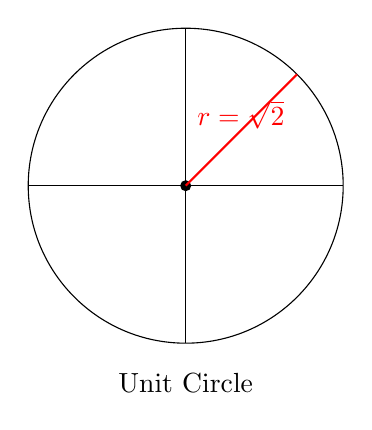
\begin{tikzpicture}
\draw (0,0) circle (2cm);
\draw (-2,0) -- (2,0);
\draw (0,-2) -- (0,2);
\fill (0,0) circle (2pt);
\node at (0,-2.5) {Unit Circle};
\draw[red, thick] (0,0) -- (1.414,1.414);
\node[red] at (0.7,0.9) {$r=\sqrt{2}$};
\end{tikzpicture}
\caption{A simple TikZ diagram}
\label{fig:tikz}
\end{figure}

\subsection{Colored Text}
\textcolor{red}{Red text}, \textcolor{blue}{blue text}, and \textcolor{green}{green text}.

\colorbox{yellow}{Text with yellow background}

\section{Page Layout and Spacing}

\subsection{Manual Spacing}
Text with various spacing:\\ 
Line break here.

\vspace{1cm}
Vertical space above this line.

\hspace{2cm}Horizontal space before this text.

\subsection{Page Breaks and Clearpage}
This section tests page layout commands.

\newpage

\section{Advanced Mathematical Constructs}

\subsection{Limits and Series}
\begin{equation}
\lim_{x \to 0} \frac{\sin x}{x} = 1
\end{equation}

\begin{equation}
\sum_{k=1}^{\infty} \frac{1}{k^2} = \frac{\pi^2}{6}
\end{equation}

\subsection{Integrals and Derivatives}
\begin{equation}
\frac{d}{dx}\left(\int_a^x f(t) dt\right) = f(x)
\end{equation}

\begin{equation}
\int_0^{\pi} \sin^n x \, dx = \begin{cases}
\frac{(n-1)!!}{n!!} \cdot \frac{\pi}{2} & \text{if } n \text{ is even} \\
\frac{(n-1)!!}{n!!} \cdot 2 & \text{if } n \text{ is odd}
\end{cases}
\end{equation}

\section{Bibliography and References}

According to \cite{knuth1984} and \cite{lamport1994}, \LaTeX{} provides excellent typesetting capabilities.

\begin{thebibliography}{99}
\bibitem{knuth1984} Donald E. Knuth. \textit{The \TeX{}book}. Addison-Wesley, 1984.
\bibitem{lamport1994} Leslie Lamport. \textit{\LaTeX{}: A Document Preparation System}. Addison-Wesley, 1994.
\end{thebibliography}

\appendix

\section{Appendix: Additional Test Cases}
\label{sec:appendix}

This appendix contains additional test structures to further exercise the DVI parser.

\subsection{Nested Math Environments}
\begin{equation}
\begin{aligned}
f(x) &= \sum_{n=0}^{\infty} \frac{f^{(n)}(a)}{n!}(x-a)^n \\
&= f(a) + f'(a)(x-a) + \frac{f''(a)}{2!}(x-a)^2 + \cdots
\end{aligned}
\end{equation}

\subsection{Complex Table Structure}
\begin{longtable}{|p{2cm}|p{3cm}|p{4cm}|p{3cm}|}
\caption{Long table spanning multiple pages} \\
\hline
Column 1 & Column 2 & Column 3 & Column 4 \\
\hline
\endfirsthead
\hline
Column 1 & Column 2 & Column 3 & Column 4 \\
\hline
\endhead
\hline
\endfoot
\hline
\endlastfoot

Row 1 & Data A & More complex data with math $\alpha + \beta$ & Final column \\
Row 2 & Data B & Information with \textbf{bold} and \textit{italic} & Another entry \\
Row 3 & Data C & \code{Code snippet here} & Last entry \\
\end{longtable}

\end{document}